\documentclass[xcolor=dvipsnames]{beamer}
\usetheme{Darmstadt}
\setbeamertemplate{navigation symbols}{}
%\setbeamertemplate{headline}{}
%\setbeamertemplate{frametitle}{\insertpagenumber}
\setbeamertemplate{footline}[frame number]

\usepackage[english]{babel}
\usepackage[cp1250]{inputenc}

\usepackage{array}

\usepackage{hyperref}
%\hypersetup{colorlinks, linkcolor=black}

\usepackage{times}
\usepackage[T1]{fontenc}


\title{Semantic Annotation Semantically:\\Using a~Shareable Extraction Ontology \\and a Reasoner}

\author[D�dek]
{Jan D�dek \and Peter Vojt�}

\institute[MFF UK]
{
Department of Software Engineering, Faculty of Mathematics and Physics, Charles University in Prague, Czech Republic
}

\date[SAIAW WI 2009]
{SEMAPRO 2011\\The Fifth International Conference on Advances in~Semantic Processing\\
November 20-25, 2011, Lisbon, Portugal}



\begin{document}

\begin{frame}
  \titlepage
\end{frame}



\begin{frame}{Outline}
  \tableofcontents
\end{frame}


\section{Introduction} 
\subsection{Semantic Annotation} 
\begin{frame}{Semantic Annotation of Text (Problem)}  
\begin{itemize}
	\item Let's have a text describing an acquisition event.
	\medskip
	\framebox{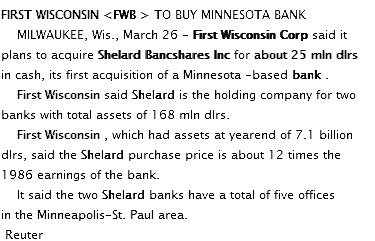
\includegraphics[width=0.6\hsize]{img/acquisitions_plain.png}}
	\item What was the object of the acquisition?
	\item Who was the buyer?
	\item What was the deal amount?
\end{itemize}
\end{frame}

\begin{frame}{Semantic Annotation of Text (Solution)}  
\begin{itemize}
	\item Well, there are Information Extraction tools that can identify and extract such information.
	\begin{itemize}
		\item Of course not 100\% accurete...
	\end{itemize}
	\medskip
	\framebox{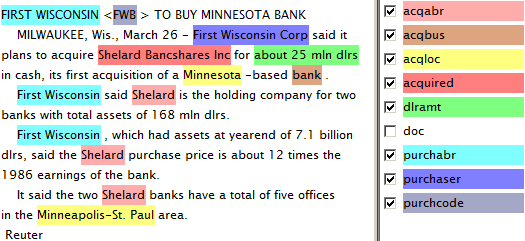
\includegraphics[width=0.85\hsize]{img/acquisitions_annotated.png}}
	\item The tools can also interpret such information in terms of a \alert{Semantic Web Ontology}.
\end{itemize}
\end{frame}

\subsection{Extraction Ontologies} 
\begin{frame}{Extraction Ontology}  
\begin{itemize}
	\item And even more! 
	\item The knowledge (extraction model) used in the extraction process can itself be saved in an ontology.
	\begin{itemize}
		\item So called Extraction Ontology
	\end{itemize}
	\bigskip
	\item D.~W. Embley, ``Toward semantic understanding: an approach based on \alert{information
  extraction ontologies},'' in \emph{ADC '04}.\hskip 1em plus 0.5em minus
  0.4em\relax Darlinghurst: ACS, 2004, pp. 3--12.
	\item M.~{Labsk\'{y} et al.}, ``{The Ex Project: Web Information Extraction Using
  \alert{Extraction Ontologies}},'' in \emph{Knowledge Discovery Enhanced with Semantic
  and Social Information}, ser. Studies in Comput. Intellig.\hskip 1em plus
  0.5em minus 0.4em\relax Springer, 2009, vol. 220, pp. 71--88.
\end{itemize}
\end{frame}

\begin{frame}{Are Such Extraction Ontologies Shareable?}  
\setbeamercolor{block title}{bg=OliveGreen}
\begin{block}{Question}
\begin{itemize}
	\item But are these Extraction Ontologies \alert{shareable}? 
	\bigskip
	\item Is it possible to use them \alert{outside} of the original tool?
\end{itemize}
\end{block}
\definecolor{MyBrown}{rgb}{0.5,0.5,0}
\setbeamercolor{block title}{bg=MyBrown}
\begin{block}{Answer}
? ...
\end{block}
\end{frame}

\begin{frame}{Example [Embley]}  
	\framebox{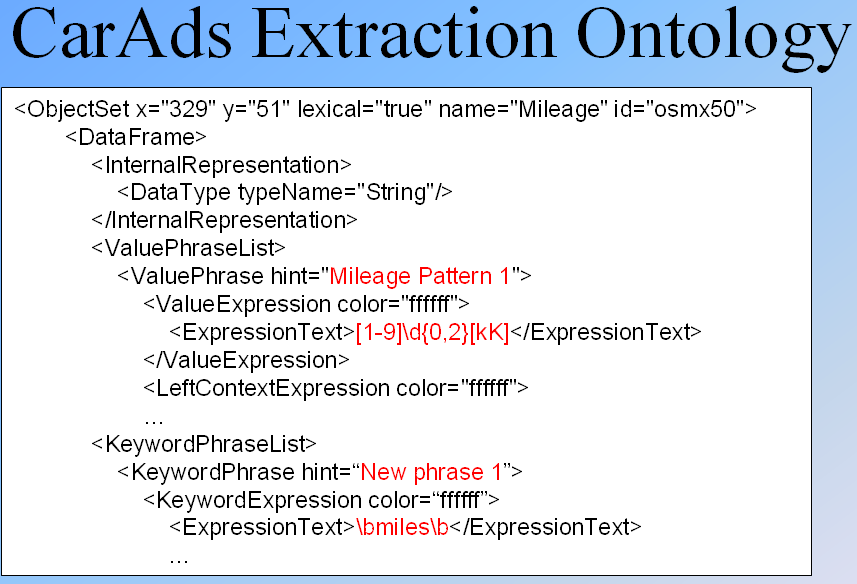
\includegraphics[width=0.85\hsize]{img/EO_car_Ad.png}}
	{\footnotesize\url{http://www.deg.byu.edu/presentations/ColloqSemanticUnderstanding.Jun2006.ppt}}
\end{frame}

\begin{frame}{Example [Labsk\'{y}]}  
	\centerline{\framebox{
\includegraphics[width=1.15\hsize]{img/EO_city_name.pdf}}}
	... pattern for matching city names which will utilize large lists of known
cities.\\
	{\footnotesize\url{http://eso.vse.cz/~labsky/ex/ex_tutorial.pdf}}
\end{frame}


\begin{frame}{Are Such Extraction Ontologies Shareable?}  
\setbeamercolor{block title}{bg=OliveGreen}
\begin{block}{Question}
\begin{itemize}
	\item But are these Extraction Ontologies shareable? 
	\bigskip
	\item Is it possible to use them outside of the original tool?
\end{itemize}
\end{block}
\setbeamercolor{block title}{bg=BrickRed}
\begin{block}{Answer}
\textbf{Not yet.}
\\Although they are conceptually modeled, the native tool is the only tool capable of interpretation of these models (ontologies).
\end{block}
\end{frame}


\section{Semantic Annotation Semantically} 
\subsection{Shareable Extraction Ontologies}
\frame{\tableofcontents[currentsection,currentsubsection]} 
\begin{frame}{Our Idea: Shareable Extraction Ontologies}
\begin{itemize}
	\item \textbf{Publish} your extraction ontology on the web and \textbf{anybody can use it with a standard reasoner}!
	\bigskip
	\item How this can be done?
	\bigskip
	\item Can a reasoner process textual reports?
\end{itemize}
\end{frame}

\subsection{Using Semantic Web Reasoners} 
\begin{frame}{Text Processing by a Reasoner}
\begin{itemize}
	\item Can a reasoner process textual reports?
	\bigskip
	\item Well, not from the beginning :-(
	\bigskip
	\item Semantic Web reasoners work only with Semantic Web ontologies.\\
	(Not with textual documents)
	\item They can read RDF \& OWL files.
	\item And also XHTML and XML files, but ...	
	\begin{itemize}
		\item But only the semantic part provided by \alert{RDFa} annotations or by a \alert{GRDDL} transformation.
	\end{itemize}
	\bigskip
	\item So we need some preprocessing...
\end{itemize}
\end{frame}

\subsection{Document Ontologies}
\begin{frame}{Document Ontologies}
\begin{itemize}
	\item ...we need some \alert{preprocessing}.
	\item That will convert a (textual) document to a ontology.
	\medskip
	\item \alert{TXT} (PDF, HTML) $\rightarrow$ \alert{RDF} (OWL)
	\medskip
	\item Document $\rightarrow$ Document Ontology (reasoner readable)
	\medskip
	\item We call the ontological representation of a document a \alert{Document Ontology}.
	\medskip
	\item Document Ontology contains:	
	\begin{itemize}
		\item All words of a document
		\item Other units necessary for: 
		\begin{itemize}
			\item Information Extraction
			\item Document reconstruction \\(Document Ontology $\rightarrow$ Document)
		\end{itemize}
	\end{itemize}
\end{itemize}
\end{frame}

\begin{frame}{From now the idea is strait forward!}
\begin{itemize}
	\item The \textbf{semantics of the Extraction Model} has to be converted to the \textbf{semantics of the Extraction Ontology}.
	\item A reasoner can then \alert{interpret} the Extraction Ontology \alert{in the same way} as the original tool would interpret the Extraction Model.
	\item Application of the Extraction Ontology on the Document Ontology by a reasoner will result in ``\alert{Annotated Document Ontology}''
	\begin{itemize}
		\item Annotated Document can be reconstructed from it.
	\end{itemize}
\end{itemize}
\end{frame}

\section{Our Case: Dependency Parsed Text} 
\frame{\tableofcontents[currentsection]} 
\subsection{System Architecture}

\begin{frame}{Information Extraction Engine}
\begin{columns}
\column{.35\textwidth}
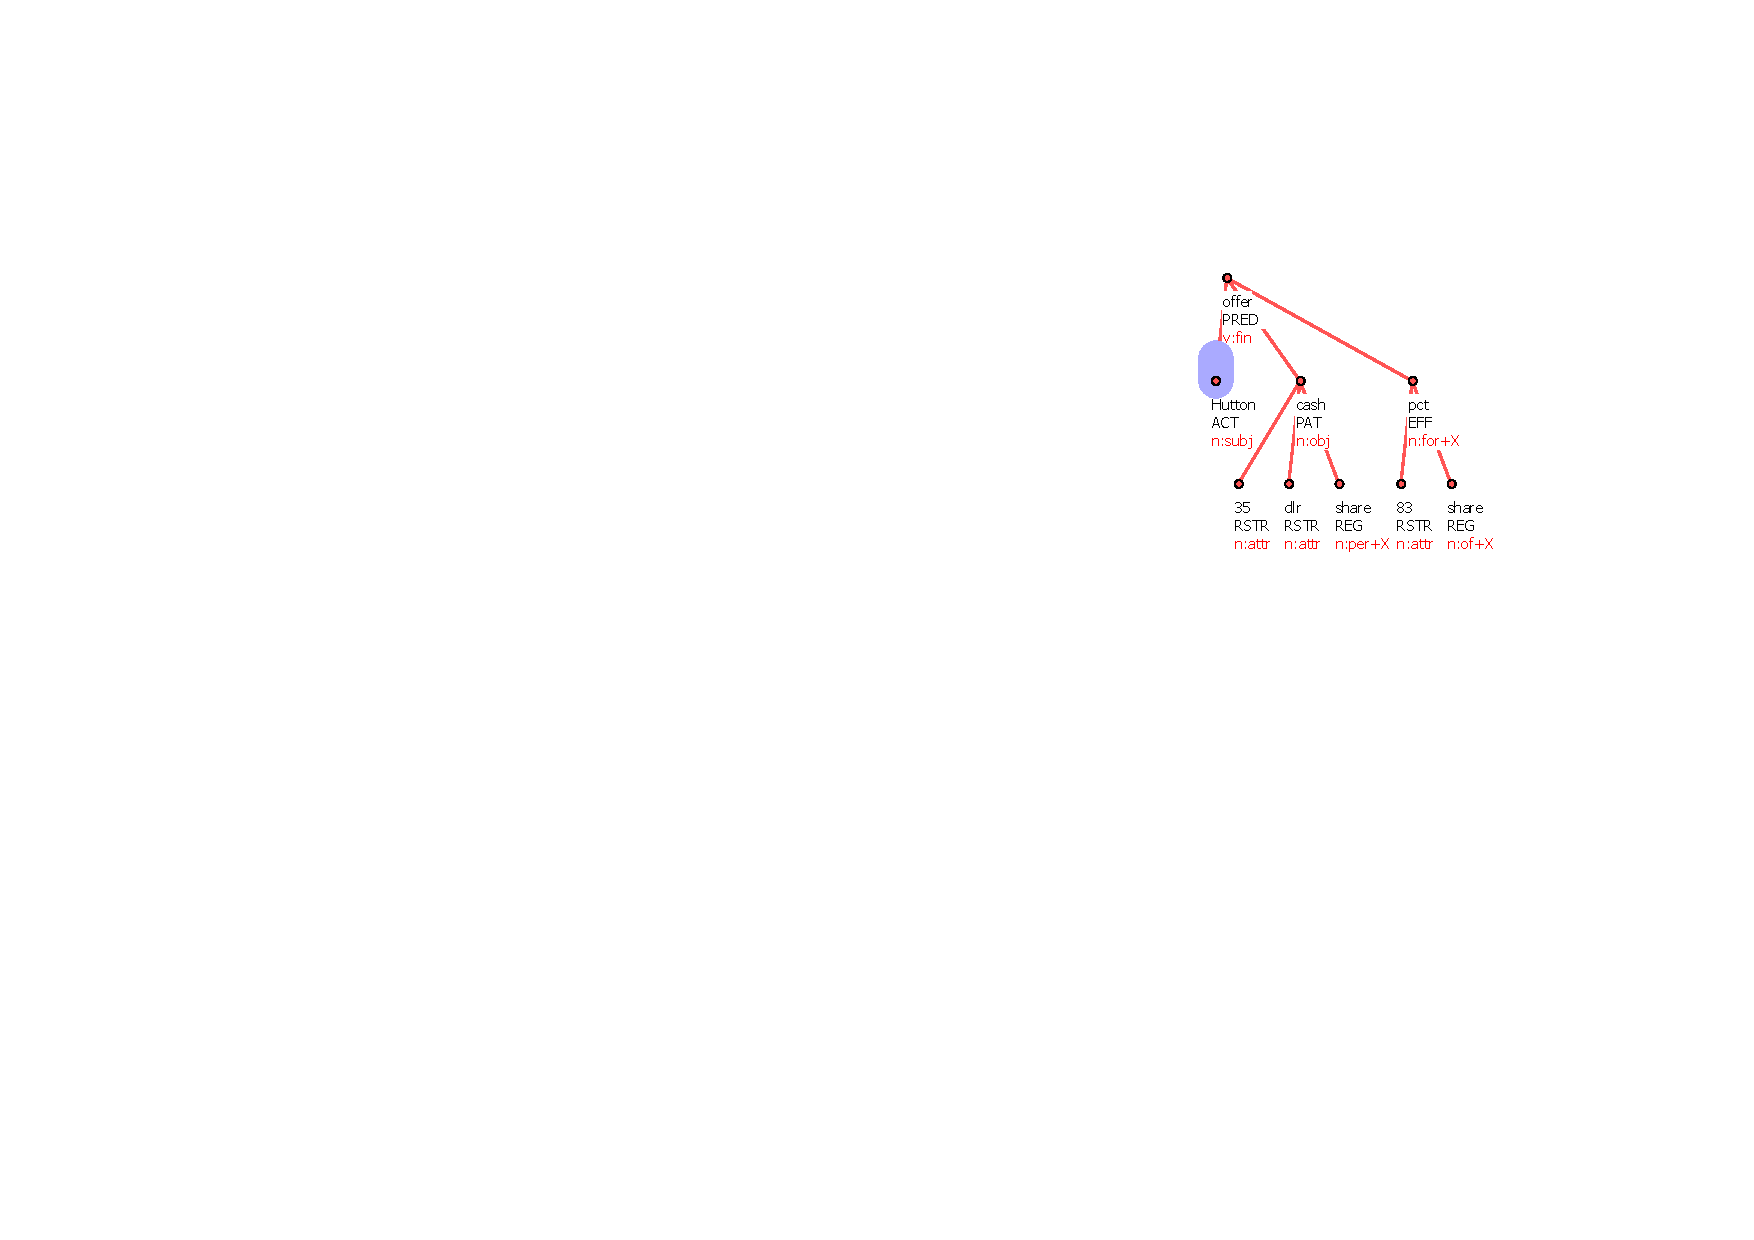
\includegraphics[width=1.1\hsize]{../img/tree.pdf}
\\
{\footnotesize``Hutton is offering 35 dlrs cash per share for 83 pct of the shares.''}
\column{.67\textwidth}
\begin{itemize}
	\item Based on dependency parsing
	\item \alert{Linguistic trees}
	\begin{itemize}
		\item Transfered to Document Ontology
	\end{itemize}
	\item Extraction rules	
	\begin{itemize}
		\item Tree patterns
	\end{itemize}
	\item \alert{Machine learning} of rules using \\Inductive Logic Programming (ILP)
	\begin{itemize}
		\item It works -- really :-)
		\item See e.g. [8] (self citation)
	\end{itemize}
	\item Rules can be also handcrafted.
	\bigskip
	\item \underline{These extraction rules can be \alert{directly}} \underline{\alert{exported to ontology} using SWRL!}
\end{itemize}
\end{columns}
\end{frame} 

\begin{frame}{System Architecture}
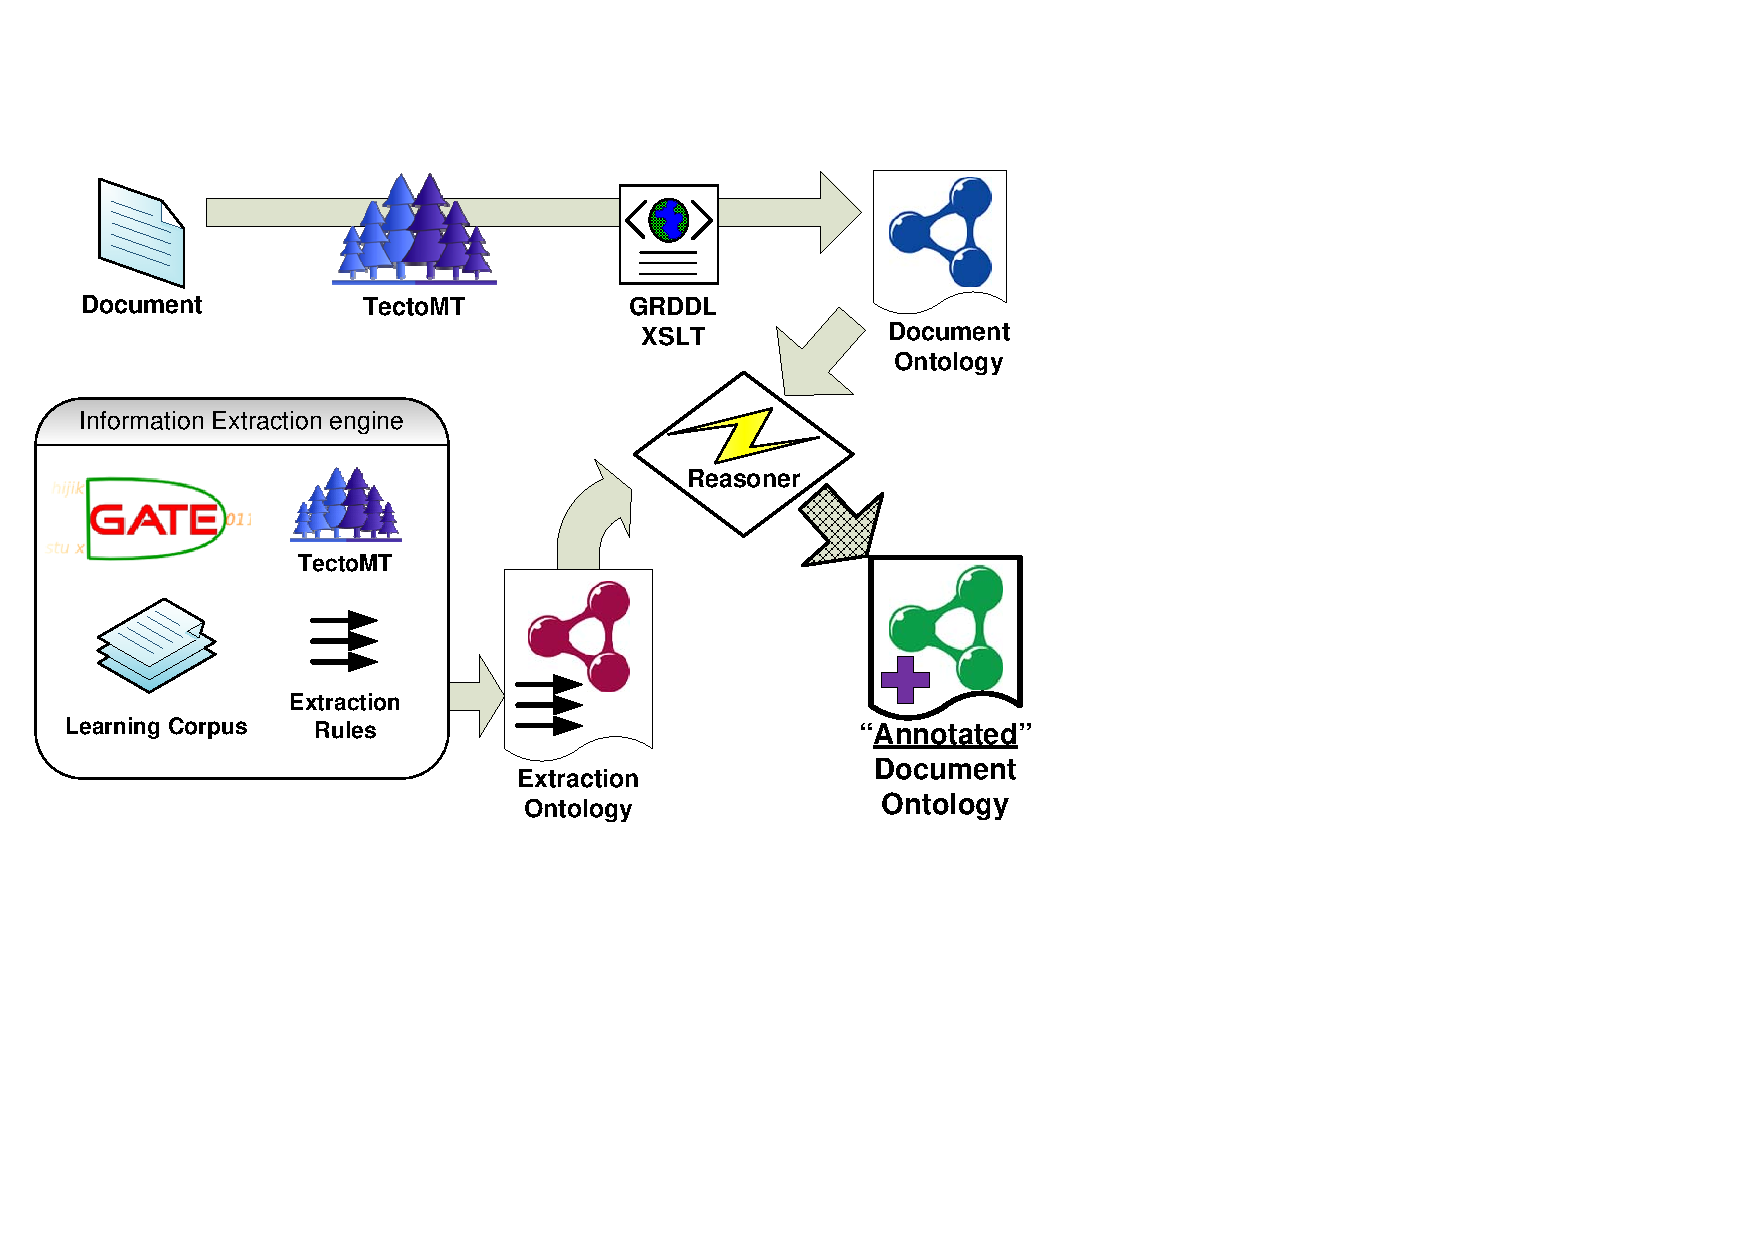
\includegraphics[width=\hsize]{../img/semantic_rules_app_schema.pdf}
\end{frame} 


\begin{frame}[fragile]{Examples of native extraction rules}
\footnotesize
[Rule 1] [Pos cover = 23 Neg cover = 6]\\
\verb@mention_root(acquired,A) :-@\\
\verb@   'lex.rf'(B,A), t_lemma(B,'Inc'),@\\
\verb@   tDependency(C,B), tDependency(C,D),@\\
\verb@   formeme(D,'n:in+X'), tDependency(E,C).@
\smallskip\newline
[Rule 11] [Pos cover = 25 Neg cover = 6]\\
\verb@mention_root(acquired,A) :-@\\
\verb@   'lex.rf'(B,A), t_lemma(B,'Inc'),@\\
\verb@   tDependency(C,B), formeme(C,'n:obj'), @\\
\verb@   tDependency(C,D), functor(D,'APP').@
\smallskip\newline
[Rule 75] [Pos cover = 14 Neg cover = 1]\\
\verb@mention_root(acquired,A) :-@\\
\verb@   'lex.rf'(B,A), t_lemma(B,'Inc'),@\\
\verb@   functor(B,'APP'), tDependency(C,B), @\\
\verb@   number(C,pl).@
\end{frame} 


\subsection{Extraction Ontology Construction} 
\frame{\tableofcontents[currentsection,currentsubsection]} 
\begin{frame}[plain]
SWRL (OWL/XML) Representation
\medskip
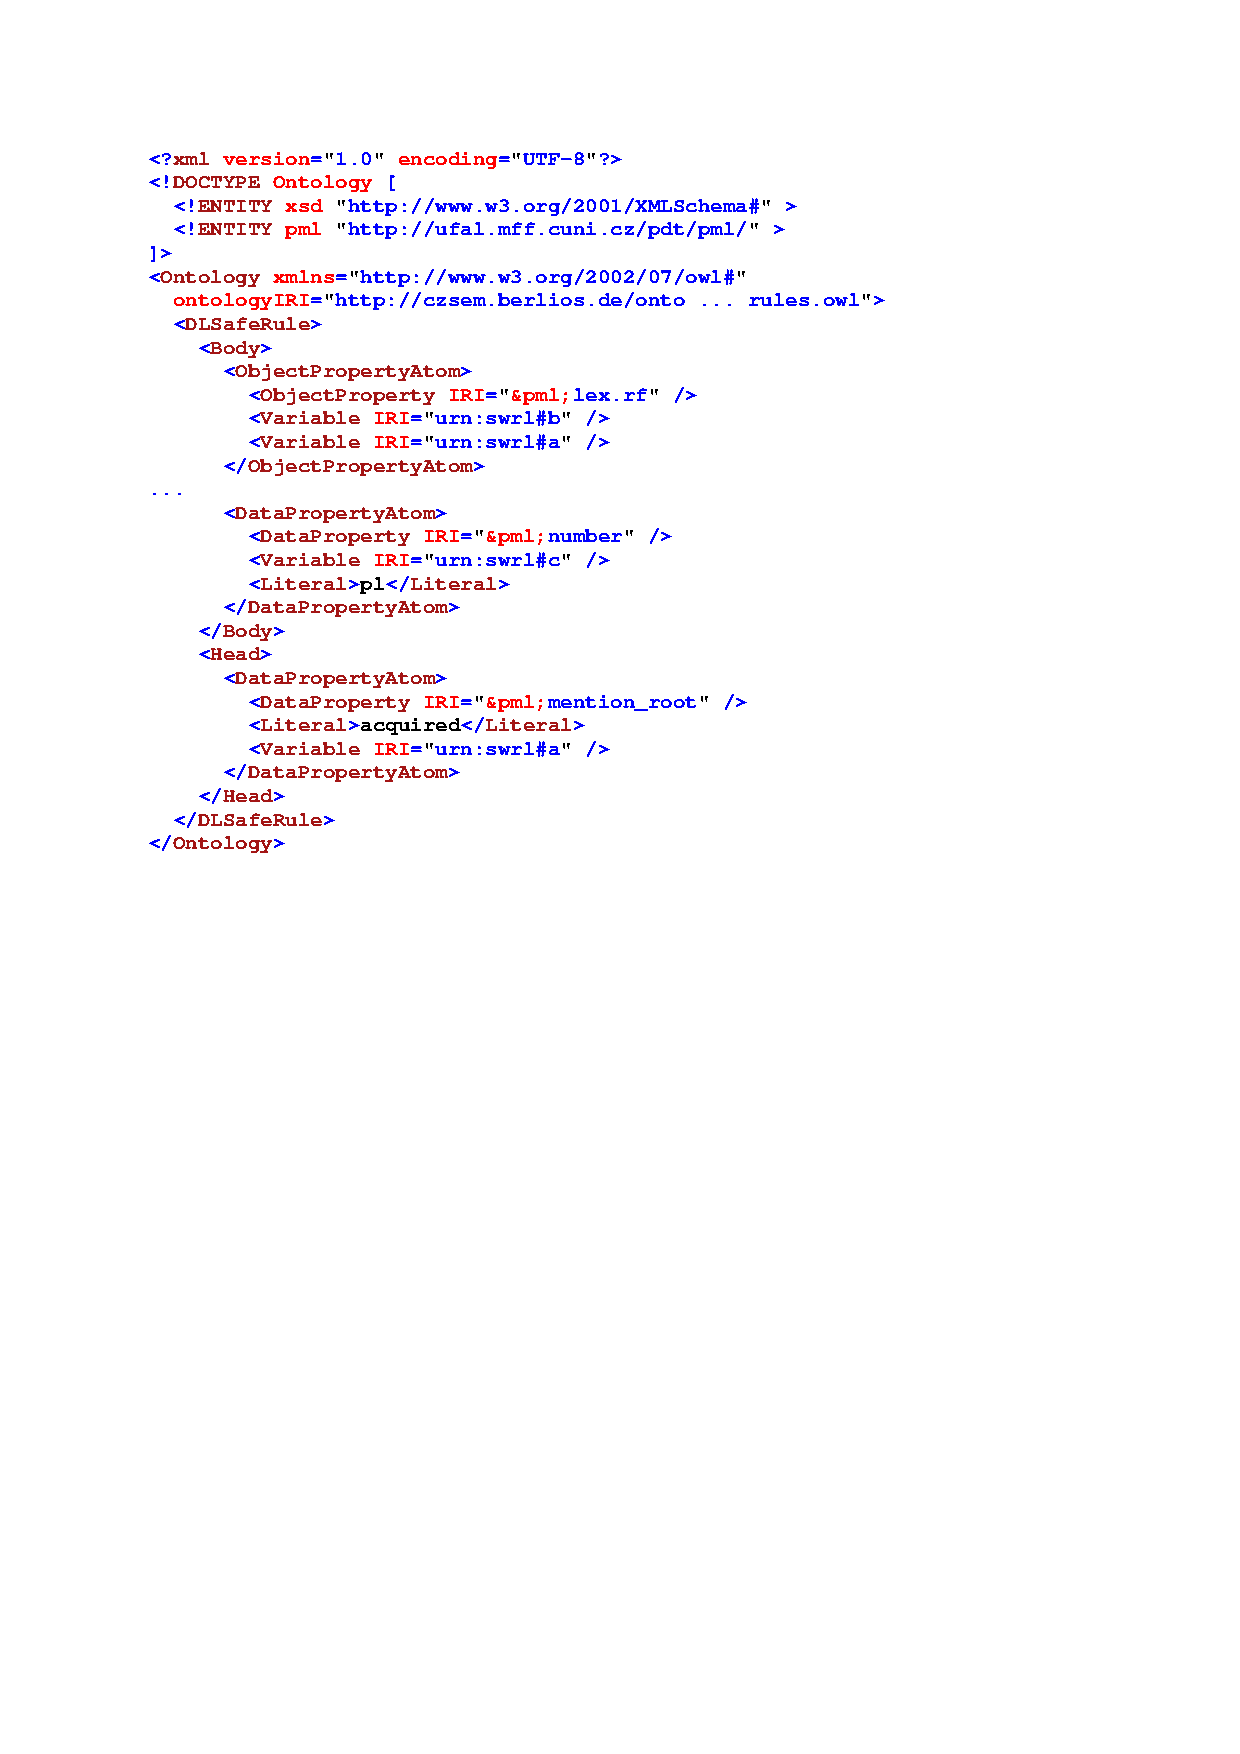
\includegraphics[width=0.8\hsize]{../img/rules_owl_xml.pdf}
\end{frame} 

\begin{frame}[fragile]{The same in Jena rules format}
\begin{verbatim}
@prefix pml: <http://ufal.mff.cuni.cz/pdt/pml/>.
[rule-75:  
        ( ?b pml:lex.rf ?a )
        ( ?c pml:tDependency ?b )
        ( ?b pml:functor 'APP' )
        ( ?c pml:number 'pl' )
        ( ?b pml:t_lemma 'Inc' )
     -> 
        ( ?a pml:mention_root 'acquired' )
]
\end{verbatim}
\end{frame} 


\subsection{Performance Evaluation} 
\frame{\tableofcontents[currentsection,currentsubsection]} 
\begin{frame}{Datasets \& Reasoners}
\centerline{
\begin{tabular}{|r||l|l|b{7mm}|b{7mm}|b{7mm}|}
\hline
\alert{dataset} & domain & language & num of files &  data size (MB) &  num of rules  \\
\hline
\hline
\textbf{czech\_fireman} & accidents & Czech &  50 &  16 &  2\\
\hline
\textbf{acquisitions} & finance & English &  600 &  126 &  113\\
\hline
\end{tabular}
}
\bigskip
\centerline{
\begin{tabular}{|r||r|r||r|r|}
\hline
\alert{reasoner} & \textbf{czech\_fireman} & stdev & \textbf{acquisitions-v1.1} & stdev\\
\hline
\hline
\textbf{Jena} & 161 s & 0.226 & 1259 s & 3.579\\
\hline
\textbf{HermiT} & 219 s & 1.636 & $\gg$ 13 hours & \\
\hline
\textbf{Pellet} & 11 s & 0.062 & 503 s & 4.145\\
\hline
\textbf{FaCT++} & \multicolumn{4}{|c|}{Does not support rules.}\\
\hline
\end{tabular}
}
\begin{itemize}
	\item How poor is the poor performance? :-)
\end{itemize}
\end{frame}

\section{Conclusion} 
\begin{frame}{Conclusion}
\begin{itemize}
	\item Idea of Shareable Extraction Ontologies presented		
	\begin{itemize}
		\item With the \alert{drawback} of the necessity of document \alert{preprocessing} (TXT $\rightarrow$ RDF)
	\end{itemize}
	\item Realization of the idea demonstrated by adaptation of our IE system 
	\item Performance \alert{evaluation} experiment done 
	\begin{itemize}
		\item Poor performance (as expected)
		\item But bearable
	\end{itemize}
	\item New public OWL (+SWRL) reasoning \alert{benchmark} created as a side effect
\end{itemize}
\end{frame}

\subsection{Future Work} 
\begin{frame}{Future Work}
\begin{itemize}
	\item \alert{Compare} the performance with rules translated to \alert{SPARQL}	
	\begin{itemize}
		\item Increased performance could be expected 
	\end{itemize}
	\smallskip
	\item Annotated Document Ontologies $\rightarrow$	\alert{Fact Ontologies}
	\begin{itemize}
		\item Data integration and duplicity of information issues
		\item Technological problems: creating new individuals during (safe) reasoning 
	\end{itemize}
	\smallskip
	\item General Shareable Extraction Ontology creation \alert{guidelines}
	\vspace{-4mm}
	\begin{itemize}
		\item E.g. how to encode a gazetteer list this way
	\end{itemize}
\end{itemize}
\end{frame}

\begin{frame}{Thank you for your attention!}
Questions?
\end{frame}


\end{document}
